\documentclass[12pt, titlepage]{article}

\usepackage{fullpage}
\usepackage[round]{natbib}
\usepackage{multirow}
\usepackage{booktabs}
\usepackage{tabularx}
\usepackage{graphicx}
\usepackage{float}
\usepackage{hyperref}
\hypersetup{
    colorlinks,
    citecolor=blue,
    filecolor=black,
    linkcolor=red,
    urlcolor=blue
}

\usepackage{tikz}
\usetikzlibrary{positioning, arrows.meta, shadows, trees}

\input{../../Comments.text}
\input{../../Common.text}

\newcounter{acnum}
\newcommand{\actheacnum}{AC\theacnum}
\newcommand{\acref}[1]{AC\ref{#1}}

\newcounter{ucnum}
\newcommand{\uctheucnum}{UC\theucnum}
\newcommand{\uref}[1]{UC\ref{#1}}

\newcounter{mnum}
\newcommand{\mthemnum}{M\themnum}
\newcommand{\mref}[1]{M\ref{#1}}

\begin{document}

\title{Module Guide for \progname{}} 
\author{\authname}
\date{\today}

\maketitle

\pagenumbering{roman}

\section{Revision History}

\begin{tabularx}{\textwidth}{p{3cm}p{2cm}X}
\toprule {\bf Date} & {\bf Version} & {\bf Notes}\\
\midrule
2026-03-23 & 1.0 & Initial MG/MIS presentation draft\\
2026-04-02 & 1.1 & Formalized 8-module hierarchy\\
2026-04-07 & 1.2 & Reviewer's edit (Yibing Mei and Dr. Smith)\\
2026-04-15 & 1.3 & Final-doc consistency pass: added Hardware/Behaviour-Hiding subsection headers in Section 6; corrected module-to-requirement traceability (Table~\ref{TblRT}) for R1--R5\\
2026-04-15 & 1.4 & Final Documentation release for CAS 741\\
2026-04-20 & 1.5 & Moved M8 (Signal Smoothing) from Behaviour-Hiding to Software Decision; Kalman-filter algorithm is not in the SRS (AC4).\\
2026-04-20 & 1.6 & Aligned \S6 prose and Table~\ref{TblRT} with M8's Software-Decision classification (removed M8 from the R2 trace; M8 traces to AC4 only).\\
\bottomrule
\end{tabularx}

\newpage

\section{Reference Material}

This section records information for easy reference. 

\subsection{Abbreviations and Acronyms}

\renewcommand{\arraystretch}{1.2}
\begin{tabular}{l l} 
  \toprule		
  \textbf{symbol} & \textbf{description}\\
  \midrule 
  AC & Anticipated Change\\
  DAG & Directed Acyclic Graph \\
  M & Module \\
  MG & Module Guide \\
  OS & Operating System \\
  R & Requirement\\
  SC & Scientific Computing \\
  SRS & Software Requirements Specification\\
  \progname & Explanation of program name\\
  UC & Unlikely Change \\
  \bottomrule
\end{tabular}\\

\newpage

\tableofcontents

\listoftables

\listoffigures

\newpage

\pagenumbering{arabic}

\section{Introduction}

Decomposing a system into modules is a commonly accepted approach to developing
software.  A module is a work assignment for a programmer or programming
team~\citep{ParnasEtAl1984}.  We advocate a decomposition
based on the principle of information hiding~\citep{Parnas1972a}.  This
principle supports design for change, because the ``secrets'' that each module
hides represent likely future changes.  Design for change is valuable in SC,
where modifications are frequent, especially during initial development as the
solution space is explored.  

Our design follows the rules layed out by \citet{ParnasEtAl1984}, as follows:
\begin{itemize}
\item System details that are likely to change independently should be the
  secrets of separate modules.
\item Each data structure is implemented in only one module.
\item Any other program that requires information stored in a module's data
  structures must obtain it by calling access programs belonging to that module.
\end{itemize}

After completing the first stage of the design, the Software Requirements
Specification (SRS), the Module Guide (MG) is developed~\citep{ParnasEtAl1984}. The MG
specifies the modular structure of the system and is intended to allow both
designers and maintainers to easily identify the parts of the software.  The
potential readers of this document are as follows:

\begin{itemize}
\item New project members: This document can be a guide for a new project member
  to easily understand the overall structure and quickly find the
  relevant modules they are searching for.
\item Maintainers: The hierarchical structure of the module guide improves the
  maintainers' understanding when they need to make changes to the system. It is
  important for a maintainer to update the relevant sections of the document
  after changes have been made.
\item Designers: Once the module guide has been written, it can be used to
  check for consistency, feasibility, and flexibility. Designers can verify the
  system in various ways, such as consistency among modules, feasibility of the
  decomposition, and flexibility of the design.
\end{itemize}

The rest of the document is organized as follows. Section
\ref{SecChange} lists the anticipated and unlikely changes of the software
requirements. Section \ref{SecMH} summarizes the module decomposition that
was constructed according to the likely changes. Section \ref{SecConnection}
specifies the connections between the software requirements and the
modules. Section \ref{SecMD} gives a detailed description of the
modules. Section \ref{SecTM} includes two traceability matrices. One checks
the completeness of the design against the requirements provided in the SRS. The
other shows the relation between anticipated changes and the modules. Section
\ref{SecUse} describes the use relation between modules.

\section{Anticipated and Unlikely Changes} \label{SecChange}

This section lists possible changes to the system. According to the likeliness
of the change, the possible changes are classified into two
categories. Anticipated changes are listed in Section \ref{SecAchange}, and
unlikely changes are listed in Section \ref{SecUchange}.

\subsection{Anticipated Changes} \label{SecAchange}

Anticipated changes are the source of the information that is to be hidden
inside the modules. Ideally, changing one of the anticipated changes will only
require changing the one module that hides the associated decision. The approach
adapted here is called design for
change.

\begin{description}
\item[\refstepcounter{acnum} \actheacnum \label{acHardware}:] The specific
  hardware on which the software is running (CPU/GPU vs. NPU).
\item[\refstepcounter{acnum} \actheacnum \label{acMLModel}:] The specific machine learning model used for pose estimation (MediaPipe, MoveNet, HRNet).
\item[\refstepcounter{acnum} \actheacnum \label{acExercise}:] The logic and thresholds for different exercise types (Squats, Bicep Curls).
\item[\refstepcounter{acnum} \actheacnum \label{acSmoothing}:] The algorithm used for signal noise reduction (Kalman Filter vs. Savitzky-Golay).
\item[\refstepcounter{acnum} \actheacnum \label{acInputFormat}:] The format of the initial video data (Base64 vs. Binary Buffers).
\item[\refstepcounter{acnum} \actheacnum \label{acFeedbackFreq}:] The frequency and refresh rate of the real-time feedback displayed to the user.
\item[\refstepcounter{acnum} \actheacnum \label{acUIBranding}:] The visual styling and branding of the user interface (colors, fonts, badge icons).
\end{description}


\subsection{Unlikely Changes} \label{SecUchange}

The module design should be as general as possible. However, a general system is
more complex. Sometimes this complexity is not necessary. Fixing some design
decisions at the system architecture stage can simplify the software design. If
these decision should later need to be changed, then many parts of the design
will potentially need to be modified. Hence, it is not intended that these
decisions will be changed.

\begin{description}
\item[\refstepcounter{ucnum} \uctheucnum \label{ucIO}:] The mathematical basis
  for biomechanical analysis (dot-product joint angle computation) is assumed to be
  a fixed, physically grounded approach that will not change.
\item[\refstepcounter{ucnum} \uctheucnum \label{ucLandmarks}:] The number of
  tracked body landmarks (33 MediaPipe Pose landmarks) is treated as fixed.
\end{description}

\section{Module Hierarchy} \label{SecMH}

This section provides an overview of the module design. Modules are summarized
in a hierarchy decomposed by secrets in Table \ref{TblMH}. The modules listed
below, which are leaves in the hierarchy tree, are the modules that will
actually be implemented.

\begin{description}
\item [\refstepcounter{mnum} \mthemnum \label{m1}:] Video Input Module
\item [\refstepcounter{mnum} \mthemnum \label{m2}:] Display Output Module
\item [\refstepcounter{mnum} \mthemnum \label{m3}:] Video Formatting Module
\item [\refstepcounter{mnum} \mthemnum \label{m4}:] Pose Tracking Module
\item [\refstepcounter{mnum} \mthemnum \label{m5}:] Kinematic Engine Module
\item [\refstepcounter{mnum} \mthemnum \label{m6}:] Exercise State Module
\item [\refstepcounter{mnum} \mthemnum \label{m7}:] UI Rendering Module
\item [\refstepcounter{mnum} \mthemnum \label{m8}:] Signal Smoothing Module
\end{description}

\begin{figure}[h!]
  \centering
  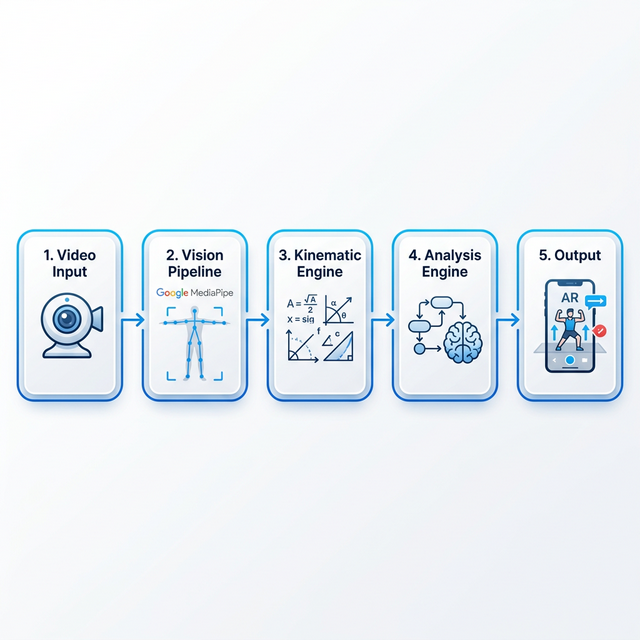
\includegraphics[width=0.8\textwidth]{architecture_diagram.png}
  \caption{System Architecture Overview}
  \label{FigArch}
\end{figure}


\begin{table}[h!]
\centering
\begin{tabular}{p{0.3\textwidth} p{0.6\textwidth}}
\toprule
\textbf{Level 1} & \textbf{Level 2}\\
\midrule

\multirow{1}{0.3\textwidth}{Hardware-Hiding} & \mref{m1}\\
\midrule

\multirow{6}{0.3\textwidth}{Behaviour-Hiding} & \mref{m2}\\
& \mref{m3}\\
& \mref{m4}\\
& \mref{m5}\\
& \mref{m6}\\
& \mref{m7}\\
\midrule

\multirow{1}{0.3\textwidth}{Software Decision} & \mref{m8} \\
\bottomrule

\end{tabular}
\caption{Module Hierarchy}
\label{TblMH}
\end{table}

\section{Connection Between Requirements and Design} \label{SecConnection}

The design of the system is intended to satisfy the requirements developed in
the SRS. In this stage, the system is decomposed into modules. The connection
between requirements and modules is listed in Table~\ref{TblRT}.

Most modules' design decisions trace directly to an SRS requirement; those
modules are classified as Behaviour-Hiding. For example, the decision to use
MediaPipe (M4) was made to satisfy the keypoint-tracking requirement (R2)
without requiring specialised hardware such as depth cameras. A few modules
hide decisions that are \emph{not} in the SRS --- for instance, the choice of
smoothing algorithm (M8) is a pure software-level decision (see AC4);
M8 therefore traces to an Anticipated Change rather than to a functional
requirement, and is classified as Software Decision.

\section{Module Decomposition} \label{SecMD}

Modules are decomposed according to the principle of ``information hiding''
proposed by \citet{ParnasEtAl1984}. The \emph{Secrets} field in a module
decomposition is a brief statement of the design decision hidden by the
module. The \emph{Services} field specifies \emph{what} the module will do
without documenting \emph{how} to do it. For each module, a suggestion for the
implementing software is given under the \emph{Implemented By} title. If the
entry is \emph{OS}, this means that the module is provided by the operating
system or by standard programming language libraries.  \emph{\progname{}} means the
module will be implemented by the \progname{} software.

Only the leaf modules in the hierarchy have to be implemented. If a dash
(\emph{--}) is shown, this means that the module is not a leaf and will not have
to be implemented.

\subsection{Hardware-Hiding Module}

\begin{description}
\item[Secrets:] The data structure and algorithm used to access hardware-level
  video capture.
\item[Services:] Serves as a virtual hardware used by the rest of the system.
  This module provides the interface between the hardware and the behaviour of
  the system.
\item[Implemented By:] Browser/OS
\end{description}

\subsubsection{Video Input Module (\mref{m1})}
\begin{description}
\item[Secrets:] The data structure and implementation used to capture raw video frames from the webcam.
\item[Services:] Provides a stream of image data to the system.
\item[Implemented By:] Browser/OS
\end{description}

\subsection{Behaviour-Hiding Module}

\begin{description}
\item[Secrets:] The contents of the required behaviours.
\item[Services:] Includes programs that provide externally visible behaviour of
  the system as specified in the SRS. This module serves as a communication
  layer between the hardware-hiding module and the software decision module.
\item[Implemented By:] FitCoachAR
\end{description}

\subsubsection{Display Output Module (\mref{m2})}
\begin{description}
\item[Secrets:] The logic for rendering the AR skeleton and badge overlays on the screen.
\item[Services:] Displays the processed video with visual feedback to the user.
\item[Implemented By:] Browser/three.js APIs
\end{description}

\subsubsection{Video Formatting Module (\mref{m3})}
\begin{description}
\item[Secrets:] The encoding and decoding algorithms used for network transmission.
\item[Services:] Converts raw image frames into transportable formats (e.g., Base64/JPEG).
\item[Implemented By:] FitCoachAR
\end{description}

\subsubsection{Exercise State Module (\mref{m6})}
\begin{description}
\item[Secrets:] The state machine logic and repetition counting thresholds.
\item[Services:] Tracks exercise progress and increments repetition count.
\item[Implemented By:] FitCoachAR
\end{description}

\subsubsection{UI Rendering Module (\mref{m7})}
\begin{description}
\item[Secrets:] The JSON schema and communication protocols for real-time feedback.
\item[Services:] Provides textual and numerical feedback (rep count, stability) to the user interface.
\item[Implemented By:] FitCoachAR
\end{description}

\subsubsection{Pose Tracking Module (\mref{m4})}
\begin{description}
\item[Secrets:] The specific machine learning models and inferencing logic for landmark extraction.
\item[Services:] Extracts 3D/2D coordinates of human joints from video frames.
\item[Implemented By:] MediaPipe (Library)
\end{description}

\subsubsection{Kinematic Engine Module (\mref{m5})}
\begin{description}
\item[Secrets:] The mathematical formulas for joint angle computation and coordinate frame transforms.
\item[Services:] Computes biomechanical metrics like joint flexion and limb alignment.
\item[Implemented By:] FitCoachAR
\end{description}

\subsection{Software Decision Module}

\begin{description}
\item[Secrets:] The design decision based on mathematical theorems, physical
  facts, or programming considerations. The secrets of this module are
  \emph{not} described in the SRS.
\item[Services:] Includes data structures and algorithms used in the system that
  do not provide direct interaction with the user.
\item[Implemented By:] --
\end{description}

\subsubsection{Signal Smoothing Module (\mref{m8})}
\begin{description}
\item[Secrets:] The filtering algorithms used to remove noise from landmark
  coordinates (e.g., Kalman filter vs.\ Savitzky--Golay). The choice of
  algorithm is not dictated by the SRS --- it is a software-decision-level
  choice made to help satisfy the NFR1 accuracy bound. This corresponds to
  anticipated change AC4.
\item[Services:] Provides a stable, non-jittery signal for downstream modules.
\item[Implemented By:] FitCoachAR
\end{description}

\section{Traceability Matrix} \label{SecTM}

This section shows two traceability matrices: between the modules and the
requirements and between the modules and the anticipated changes.

% the table should use mref, the requirements should be named, use something
% like fref
\begin{table}[H]
\centering
\begin{tabular}{p{0.2\textwidth} p{0.6\textwidth}}
\toprule
\textbf{Req.} & \textbf{Modules}\\
\midrule
R1 (R\_Input) & \mref{m1}, \mref{m3}, \mref{m7}\\
R2 (R\_Process) & \mref{m4}\\
R3 (R\_Calc) & \mref{m5}\\
R4 (R\_Verify) & \mref{m6}\\
R5 (R\_Output) & \mref{m2}, \mref{m7}\\
\bottomrule
\end{tabular}
\caption{Trace Between Requirements and Modules}
\label{TblRT}
\end{table}

\begin{table}[H]
\centering
\begin{tabular}{p{0.2\textwidth} p{0.6\textwidth}}
\toprule
\textbf{AC} & \textbf{Modules}\\
\midrule
\acref{acHardware} & \mref{m1}\\
\acref{acMLModel} & \mref{m4}\\
\acref{acExercise} & \mref{m6}, \mref{m5}\\
\acref{acSmoothing} & \mref{m8}\\
\acref{acInputFormat} & \mref{m3}\\
\bottomrule
\end{tabular}
\caption{Trace Between Anticipated Changes and Modules}
\label{TblACT}
\end{table}

\section{Use Hierarchy Between Modules} \label{SecUse}

In this section, the uses hierarchy between modules is
provided. \citet{Parnas1978} said of two programs A and B that A {\em uses} B if
correct execution of B may be necessary for A to complete the task described in
its specification. That is, A {\em uses} B if there exist situations in which
the correct functioning of A depends upon the availability of a correct
implementation of B. The use relation corresponds to Python \texttt{import}
statements in the implemented code.

The uses hierarchy is a directed acyclic graph (DAG) as illustrated below:
The uses hierarchy is a directed acyclic graph (DAG) as illustrated in Figure \ref{FigDAG}:

\begin{figure}[H]
\centering
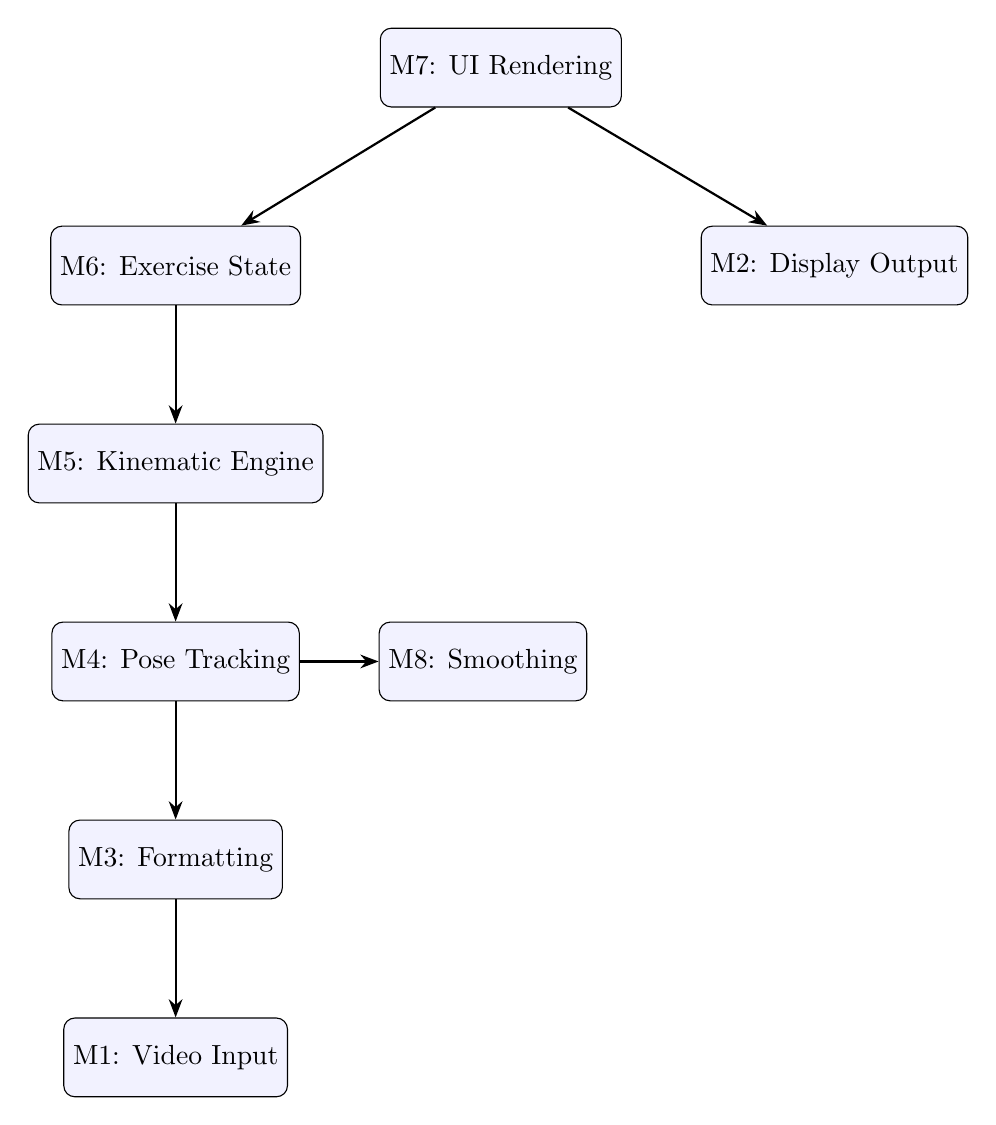
\begin{tikzpicture}[
  node distance=1.5cm and 1cm,
  box/.style={draw, rounded corners, minimum width=2.5cm, minimum height=1cm, align=center, fill=blue!5},
  arrow/.style={-Stealth, thick}
]
  % Nodes
  \node[box] (m7) {M7: UI Rendering};
  \node[box] (m6) [below left=of m7] {M6: Exercise State};
  \node[box] (m2) [below right=of m7] {M2: Display Output};
  \node[box] (m5) [below=of m6] {M5: Kinematic Engine};
  \node[box] (m4) [below=of m5] {M4: Pose Tracking};
  \node[box] (m8) [right=of m4] {M8: Smoothing};
  \node[box] (m3) [below=of m4] {M3: Formatting};
  \node[box] (m1) [below=of m3] {M1: Video Input};

  % Edges
  \draw[arrow] (m7) -- (m6);
  \draw[arrow] (m7) -- (m2);
  \draw[arrow] (m6) -- (m5);
  \draw[arrow] (m5) -- (m4);
  \draw[arrow] (m4) -- (m8);
  \draw[arrow] (m4) -- (m3);
  \draw[arrow] (m3) -- (m1);

\end{tikzpicture}
\caption{Uses Hierarchy (DAG)}
\label{FigDAG}
\end{figure}

\begin{itemize}
  \item M7 (UI Rendering) \emph{uses} M6 (Exercise State), M2 (Display Output)
  \item M6 (Exercise State) \emph{uses} M5 (Kinematic Engine)
  \item M5 (Kinematic Engine) \emph{uses} M4 (Pose Tracking)
  \item M4 (Pose Tracking) \emph{uses} M8 (Signal Smoothing), M3 (Video Formatting)
  \item M3 (Video Formatting) \emph{uses} M1 (Video Input)
\end{itemize}

%\section*{References}

\section{User Interfaces}

FitCoachAR provides two user-facing interfaces:

\begin{itemize}
  \item \textbf{Webcam Feed with AR Overlay (M2: Display Output)}: The primary
  interface is a live video feed rendered in the browser. The system draws a
  skeleton overlay on the user's body using detected landmarks, and displays
  real-time feedback badges showing the current repetition count and form
  quality scores (e.g., knee stability index, torso lean angle).

  \item \textbf{Exercise Control Panel (M7: UI Rendering)}: A sidebar panel
  allows the user to select an exercise type (Squat or Bicep Curl), start and
  stop a session, and view a summary of completed repetitions. The panel updates
  in real-time via a WebSocket connection to the backend.
\end{itemize}

\section{Database Design}

FitCoachAR does not use a persistent database in the current implementation.
All session state (rep count, current phase, smoothed angles) is maintained
in memory on the backend for the duration of a session and discarded afterward.
This is an intentional design decision to simplify the system and avoid
privacy concerns with storing biometric workout data.

\section{Timeline}

Implementation was completed as part of the CAS 741 course project.
The development schedule and task assignments are tracked via GitHub Issues
and milestones at \url{https://github.com/mmdmirh/cas741}.

\bibliographystyle {plainnat}
\bibliography{../../../refs/References}

\newpage{}

\end{document}
